\pagestyle{myFancy}
\chapter{Simulations Results}
In this chapter original results from simulations are presented.
The code used to perform such simulations is based on the code originally developed for the calculations presented in refs.~\cite{Panero:2009tv,Mykkanen:2012ri}.

\section{Rotational Invariance Restoration}
This first section has the aim to reproduce the rotational invariance restoration of~\cite{Lang:1982tj} for the continuous group $\SU(2)$ (and not for the discrete icosahedral group $\tilde{Y}$, like explained in \secref{Sec3:RotInv}).\\
This is done by evaluating the correlator of two Polyakov loops as explained in \secref{Sec2:PolyakovLoops}, computed on two different lattices with two different values of $\beta$, corresponding to two different lattice spacings.

\subsection{Simulations Setup}
The lattices are taken to be periodic in every direction, with $n_s$ sites in each space direction ($n_s=n_x=n_y=n_z$) and $n_t$ sites in the time direction.
The lattice has, therefore, $n_s^3n_t$ sites.\\
The simulations are run from a cold start, with $2500$ thermalization steps, where each Monte Carlo step is composed of $1$ heat bath step followed by $3$ overrelaxation steps.
Since the plaquette is observed to thermalize after $O(10)$ steps in preliminary simulations with both hot and cold starts, $2500$ thermalization steps are enough to ensure full thermalization.\\
After that, $20000$ measurements are taken of every possible independent correlator between two Polyakov loops, with $100$ updates between each measurement.\\
On a lattice with $n_s$ spatial sites in each direction, only couples of Polyakov loops whose distance, in each spatial direction, is $\leq n_s/2$ are independent: for example a couple of Polyakov loops extending for $n_s/2+1$ sites in a certain direction is equivalent to the hermitian conjugate of a couple extending for $n_s/2-1$ sites, because of the periodic boundary conditions (see \eqref{2:nonzeroMomPolyakov}).
But, since the Polyakov loops correlator expectation value is real, they have the same numerical value.\\
In \figref{4F:PolyakovPeriodic} is represented a graphical visualization of this fact.
\begin{figure}[!htbp]
    \centering
    \begin{subfigure}[b]{0.48\textwidth}
        \centering
        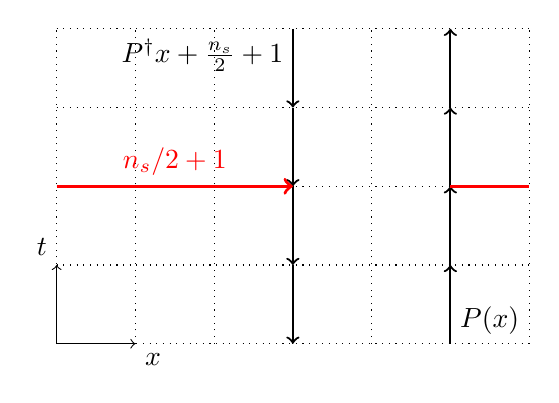
\begin{tikzpicture}
            \draw[step=1.0,dotted] (0,0) grid (6,4);
            \draw[->] (0,0) -- (1,0) node[anchor=north west]{$x$};
            \draw[->] (0,0) -- (0,1) node[anchor=south east]{$t$};
            
            \draw (5,0) node[anchor=south west]{$P(x)$};
            \draw[thick,->] (5,0) -- (5,1);
            \draw[thick,->] (5,1) -- (5,2);
            \draw[thick,->] (5,2) -- (5,3);
            \draw[thick,->] (5,3) -- (5,4);
            
            \draw (3,4) node[anchor=north east]{$P^\dagger\pr{x+\frac{n_s}{2}+1}$};
            \draw[thick,->] (3,4) -- (3,3);
            \draw[thick,->] (3,3) -- (3,2);
            \draw[thick,->] (3,2) -- (3,1);
            \draw[thick,->] (3,1) -- (3,0);
            
            \draw[very thick,red] (5,2) -- (6,2);
            \draw[very thick,red] (1.5,2) node[anchor=south]{$n_s/2+1$};
            \draw[very thick,red,->] (0,2) -- (3,2);
        \end{tikzpicture}
    \end{subfigure}
    \hfill
    \begin{subfigure}[b]{0.48\textwidth}
        \centering
        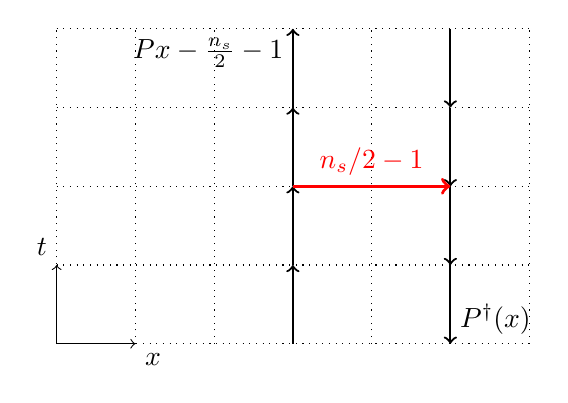
\begin{tikzpicture}
            \draw[step=1.0,dotted] (0,0) grid (6,4);
            \draw[->] (0,0) -- (1,0) node[anchor=north west]{$x$};
            \draw[->] (0,0) -- (0,1) node[anchor=south east]{$t$};
            
            \draw (5,0) node[anchor=south west]{$P^\dagger(x)$};
            \draw[thick,->] (5,4) -- (5,3);
            \draw[thick,->] (5,3) -- (5,2);
            \draw[thick,->] (5,2) -- (5,1);
            \draw[thick,->] (5,1) -- (5,0);
            
            \draw (3,4) node[anchor=north east]{$P\pr{x-\pr{\frac{n_s}{2}-1}}$};
            \draw[thick,->] (3,0) -- (3,1);
            \draw[thick,->] (3,1) -- (3,2);
            \draw[thick,->] (3,2) -- (3,3);
            \draw[thick,->] (3,3) -- (3,4);
            
            \draw[very thick,red,->] (3,2) -- (5,2);
            \draw[very thick,red] (4,2) node[anchor=south]{$n_s/2-1$};
        \end{tikzpicture}
    \end{subfigure}
    \caption{The correlator of two Polyakov loops distant $n_s/2+1$ sites (left) is equal to the hermitian conjugate of the correlator of two Polyakov loops distant $n_s/2-1$ sites (right), \ie $\expval{P(x)P^\dagger\pr{x+\frac{n_s}{2}+1}}=\expval{P\pr{x-\pr{\frac{n_s}{2}-1}}P^\dagger(x)}^\dagger$.}
    \label{4F:PolyakovPeriodic}
\end{figure}\\
Therefore, only Polyakov correlators extending from size $(0,0,0)$ to size $(n_s/2,n_s/2,n_s/2)$ are considered.
Correlators of the same size are then averaged together and the uncorrelated empirical standard deviation is computed as an estimate of the error.

\subsection{Analysis of Data}
After checking that each correlator's mean value is real (its imaginary part is compatible with $0$), these averages are used to compute the potential, in units of the lattice spacing $a$, as:
\begin{equation}
    V(x,y,z) = -\frac{1}{n_t}\ln\expval{P(0)P^\dagger(x,y,z)} \label{4:Potential}
\end{equation}
where $(x,y,z)\in\prc{(0,0,0),\dots,\pr{\frac{n_s}{2},\frac{n_s}{2},\frac{n_s}{2}}}$.
The standard deviation is computed with the usual error propagation formula.\\
Graphics like \figref{3F:LangRebbi} are obtained considering a section of the lattices used, specifically the $xy$-plane, that is done by plotting only values of $V(x,y,z=0)$.\\
In order to verify that there are no anisotropies, all the three coordinate planes are plotted in \figref{4F:PotentialPlanes}.\\
Corresponding points in each plane are compatible with each other within the standard deviation and there is no visible difference between different coordinate planes.
This justifies choosing arbitrarily one plane for each lattice.
\begin{figure}[!htbp]
    \centering
    \begin{subfigure}[t]{\textwidth}
        \centering
        \begin{subfigure}[t]{0.32\textwidth}
            \renewcommand\thesubfigure{\alph{subfigure}1}
            \includegraphics[width=\textwidth]{nt4_ns8_beta2.20/xy.png}
            \caption{$xy$-plane}
            \label{4F:PotentialPlanes48xy}
        \end{subfigure}
        \hfill
        \begin{subfigure}[t]{0.32\textwidth}
            \addtocounter{subfigure}{-1}
            \renewcommand\thesubfigure{\alph{subfigure}2}
            \includegraphics[width=\textwidth]{nt4_ns8_beta2.20/xz.png}
            \caption{$xz$-plane}
            \label{4F:PotentialPlanes48xz}
        \end{subfigure}
        \hfill
        \begin{subfigure}[t]{0.32\textwidth}
            \addtocounter{subfigure}{-1}
            \renewcommand\thesubfigure{\alph{subfigure}3}
            \includegraphics[width=\textwidth]{nt4_ns8_beta2.20/yz.png}
            \caption{$yz$-plane}
            \label{4F:PotentialPlanes48yz}
        \end{subfigure}
        \addtocounter{subfigure}{-1}
        \caption{Lattice with $n_s=4$, $n_s=8$, $\beta=2.20$.}
        \label{4F:PotentialPlanes48}
    \end{subfigure}\\
    \vspace{\baselineskip}
    \begin{subfigure}[b]{\textwidth}
        \centering
        \begin{subfigure}[b]{0.32\textwidth}
            \renewcommand\thesubfigure{\alph{subfigure}1}
            \includegraphics[width=\textwidth]{nt6_ns16_beta2.35/xy.png}
            \caption{$xy$-plane}
            \label{4F:PotentialPlanes616xy}
        \end{subfigure}
        \hfill
        \begin{subfigure}[b]{0.32\textwidth}
            \addtocounter{subfigure}{-1}
            \renewcommand\thesubfigure{\alph{subfigure}2}
            \includegraphics[width=\textwidth]{nt6_ns16_beta2.35/xz.png}
            \caption{$xz$-plane}
            \label{4F:PotentialPlanes616xz}
        \end{subfigure}
        \hfill
        \begin{subfigure}[b]{0.32\textwidth}
            \addtocounter{subfigure}{-1}
            \renewcommand\thesubfigure{\alph{subfigure}3}
            \includegraphics[width=\textwidth]{nt6_ns16_beta2.35/yz.png}
            \caption{$yz$-plane}
            \label{4F:PotentialPlanes616yz}
        \end{subfigure}
        \addtocounter{subfigure}{-1}
        \caption{Lattice with $n_s=6$, $n_s=16$, $\beta=2.35$.}
        \label{4F:PotentialPlanes616}
    \end{subfigure}
    \caption{Plots of the static quark potential in the three coordinate planes for two different lattices. The colored scale represent the potential in lattice spacing units.}
    \label{4F:PotentialPlanes}
\end{figure}
\begin{figure}[!htbp]
    \centering
    \begin{subfigure}[b]{0.48\textwidth}
        \includegraphics[width=\textwidth]{nt4_ns8_beta2.20/RotSymm.png}
        \caption{Lattice with $n_s=4$, $n_s=8$, $\beta=2.20$.}
        \label{4F:PotentialRestorationLargea}
    \end{subfigure}
    \begin{subfigure}[b]{0.48\textwidth}
        \includegraphics[width=\textwidth]{nt6_ns16_beta2.35/RotSymm.png}
        \caption{Lattice with $n_s=6$, $n_s=16$, $\beta=2.35$.}
        \label{4F:PotentialRestorationSmalla}
    \end{subfigure}
    \caption{Rotational invariance restoration of the static quark potential.}
    \label{4F:PotentialRestoration}
\end{figure}\\
In order to give a more ``complete'' view, data from \figref{4F:PotentialPlanes48xy} and \figref{4F:PotentialPlanes616xy} is reflected relative to the $x$ and $y$ axis, obtaining the plots in \figref{4F:PotentialRestoration}.\\
In both \figref{4F:PotentialPlanes} and \figref{4F:PotentialRestoration} correlators of Polyakov loops far from the origin (the ones represented by blue dots, with values of the potential $\gtrsim 1.4$) were compatible with each other.
The interesting parts of these graphics are, therefore, the dots up to the dark green shade.

\subsection{Final Remarks}
It is interesting to note the resemblance of \figref{4F:PotentialRestoration} with \figref{3F:LangRebbi}, although they are obtained in different ways and for different gauge groups.
Note also that the values of $\beta$ used in these simulations were slightly higher than the ones used in \cite{Lang:1982tj}, in order to have a smaller lattice spacing that allowed a finer determination of the potential.

\section{BCT Lattice}
